\documentclass[a4paper, 11pt]{article}
\usepackage{comment} % enables the use of multi-line comments (\ifx \fi) 
\usepackage[top = 0.5in, bottom=0.5in]{geometry}
\usepackage{color, listings, graphicx, float, booktabs, tabularx, multirow, amsmath, changepage, subcaption}

\usepackage[colorlinks=true, urlcolor=blue]{hyperref}

\definecolor{codegreen}{rgb}{0,0.6,0}
\definecolor{codegray}{rgb}{0.5,0.5,0.5}
\definecolor{codepurple}{rgb}{0.58,0,0.82}
\definecolor{backcolour}{rgb}{0.95,0.95,0.92}
 
\lstdefinestyle{mystyle}{
    backgroundcolor=\color{backcolour},   
    basicstyle=\footnotesize,
    breakatwhitespace=false,         
    breaklines=true,                 
    captionpos=b,                    
    keepspaces=true,                 
%    numbers=left,                    
%    numbersep=5pt,                  
    showspaces=false,                
    showstringspaces=false,
    showtabs=false,                  
    tabsize=1
}
\lstset{style=mystyle}

\def\changemargin#1#2{\list{}{\rightmargin#2\leftmargin#1}\item[]}
\let\endchangemargin=\endlist 

\begin{document}
\graphicspath{{./figures/}}
\noindent
\large\textbf{Kyle Salitrik (kps168)} \\
\normalsize STAT 462\\
\large{Homework 4 Report} \hfill 
%%%%%%%%%%%%%%%%%%%%%%%%%%%%%%%%%%%%%%%%%%%%%%%%%%%%%%%%%%%%%%%%%%%%
%%% SECTION: Applied
%%%%%%%%%%%%%%%%%%%%%%%%%%%%%%%%%%%%%%%%%%%%%%%%%%%%%%%%%%%%%%%%%%%%
\section*{Applied Analysis}
The following reduction was performed on the data in order to remove influential points, outliers and errors.
\begin{itemize}
	\setlength\itemsep{0em}
	\item Samples below 2\% and above 40\% body fat were excluded. The minimum was obtained through the chart on the (\href{''https://www.acefitness.org/acefit/healthy-living-article/60/112/what-are-the-guidelines-for-percentage-of-body-fat-loss''}{\underline{ACE}}) website and maximum was set to limit outliers.
	\item The minimum height accepted was cut to be over 50 inches to remove outliers.
	\item The maximum weight was also clipped to be below 300 pounds. Although the outlier may have been legitimate, it could have also been an error.
	\item Observation number 41 was removed as an influential point.
\end{itemize}

%====================================================================
\subsection*{Part A: Backward Elimination}
Beginning with the full model below, at every step the predictor with the highest p-value was removed until all predictors were below the threshold of $\alpha = 0.15$. 
\begin{align*}
	y = & \beta_0 + \beta_1\text{AbdomenC} + \beta_2\text{Weight} + \beta_3\text{Height} + \beta_4\text{NeckC} + \beta_5\text{ChestC} + \\
	& \beta_6\text{HipC} + \beta_7\text{ThighC} + \beta_8\text{KneeC} + \beta_9\text{AnkleC} + \beta_{10}\text{BicepsC} +  \\ 
	&\beta_{11}\text{ForearmC} + \beta_{12}\text{WristC} +\beta_{13}\text{Over45}+ \epsilon
\end{align*}

Through this process, the following predictors were removed in the order presented:
\begin{itemize}
	\setlength\itemsep{0em}
	\item Knee Circumference
	\item Thigh Circumference
	\item Weight
	\item Ankle Circumference
	\item Biceps Circumference
	\item Chest Circumference
	\item Forearm Circumference
	\item Hip Circumference
\end{itemize}

The final model obtained from backwards elimination is:

\begin{align*}
	y = & \beta_0 + \beta_1\text{AbdomenC} + \beta_2\text{Height} + \beta_3\text{NeckC} + \beta_4\text{WristC} + \epsilon
\end{align*}

%====================================================================
\subsection*{Part B: Forward Selection}
Starting with zero predictors, 13 models were generated (each with one of the 13 predictors) and the p-values of the new predictors were saved off. The predictor with the lowest p-value was added to the real model and the process was repeated for the 12 remaining predictors. This continued until any additional predictors had a p-value of greater than 0.15.

The following presents the order in which predictors were added:
\begin{itemize}
	\setlength\itemsep{0em}
	\item Abdomen Circumference
	\item Weight
	\item Wrist Circumference
	\item Height
\end{itemize}

The model below was then fit based on this selection:
\begin{align*}
	y = & \beta_0 + \beta_1\text{AbdomenC} + \beta_2\text{Weight} + \beta_3\text{WristC} + \beta_4\text{Height} + \epsilon
\end{align*}


%====================================================================
\subsection*{Part C: RSS, Mallow's C, AIC, and BIC Selection}
The "leaps" R package was used to exhaustively search for the best models at a set number of predictors. These results are displayed below (with the intercept term removed from the output) and were used to determine the predictors present in the corresponding models.
\begin{changemargin}{-2cm}{-2cm}
	\begin{center}
		\lstinputlisting[language={}, caption=regsubsets Function Output]{./output/leaps.txt}
	\end{center}
\end{changemargin}

Beginning with the method of model selection using adjusted R-squared values, the plot below shows that the highest value occurs at 8 betas, or 7 predictors.
\begin{figure}[H]
	\centering
	\caption{Adjusted $R^2$ Plot}
	\centerline{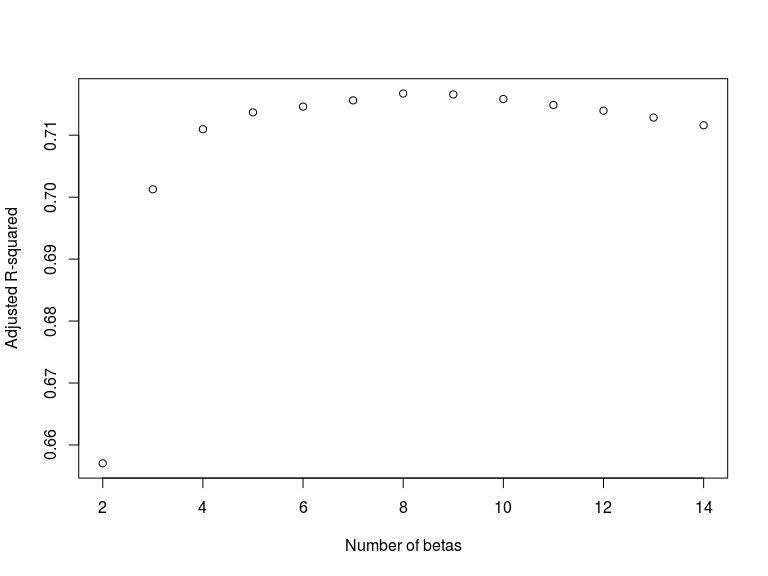
\includegraphics[width=.8\textwidth]{adj_r2.png}}
\end{figure}

Using the regsubsets output and this information, we can obtain the following model:

\begin{align*}
	y = & \beta_0 + \beta_1\text{AbdomenC} + \beta_2\text{Height} + \beta_3\text{NeckC} + \beta_4\text{ChestC} + \beta_5\text{HipC} + \\
	&\beta_6\text{ForearmC} + \beta_7\text{WristC} + \epsilon
\end{align*}

The second method of model selection explored in this section is using the Mallow's C values for a given number of predictors to determine the best model. When looking at the differences between the C values and the number of predictors, the closest fit is at $C_3$. This indicates that 4 betas (or 3 predictors) is the best model based on this method. The following plot contains the Mallow's C values for up to 13 predictors.

\begin{figure}[H]
	\centering
	\caption{Mallow's $C_p$ Plot}
	\centerline{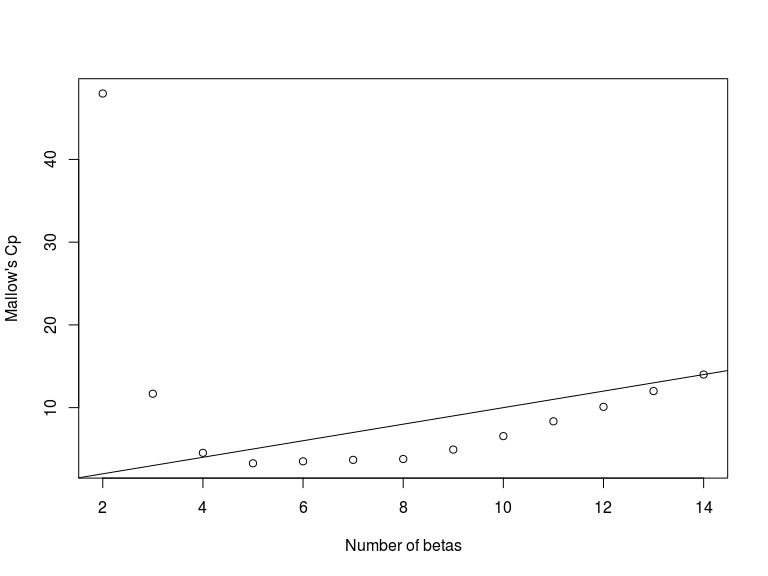
\includegraphics[width=.8\textwidth]{mallows_c.png}}
\end{figure}

Once again, using the regsubsets information the linear model below is obtained:
\begin{align*}
	y = & \beta_0 + \beta_1\text{AbdomenC} + \beta_2\text{Weight} + \beta_3\text{WristC} + \epsilon
\end{align*}

For the third method, AIC, the minimum value indicates which model is the best fit according to the metric. The plot of values and linear model can be seen below, with $p=4$. Predictors in the model were obtained from the regsubsets function.
\begin{figure}[H]
	\centering
	\caption{AIC Plot}
	\centerline{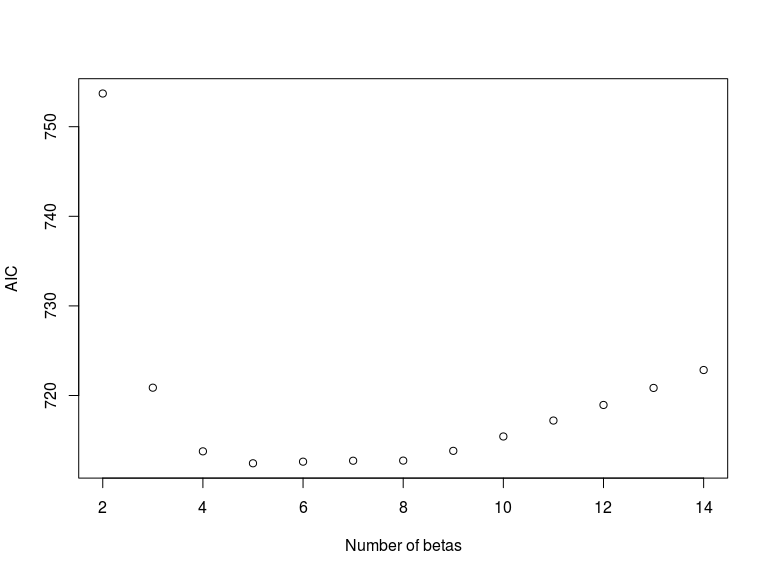
\includegraphics[width=.8\textwidth]{aic.png}}
\end{figure}

It is worth noting that the best model for $p=4$ is identical to the model obtained by backward elimination.
\begin{align*}
	y = & \beta_0 + \beta_1\text{AbdomenC} + \beta_2\text{Weight} + \beta_3\text{NeckC} + \beta_4\text{WristC} + \epsilon
\end{align*}

Finally, the execution and interpretation is similar to that of the AIC method in that the minimum value of the results corresponding to a given number of predictors indicates the number of predictors for the best fit. The number of predictors obtained here is the same as the Mallow's C values, and is therefore the same model.
\begin{figure}[H]
	\centering
	\caption{BIC Plot}
	\centerline{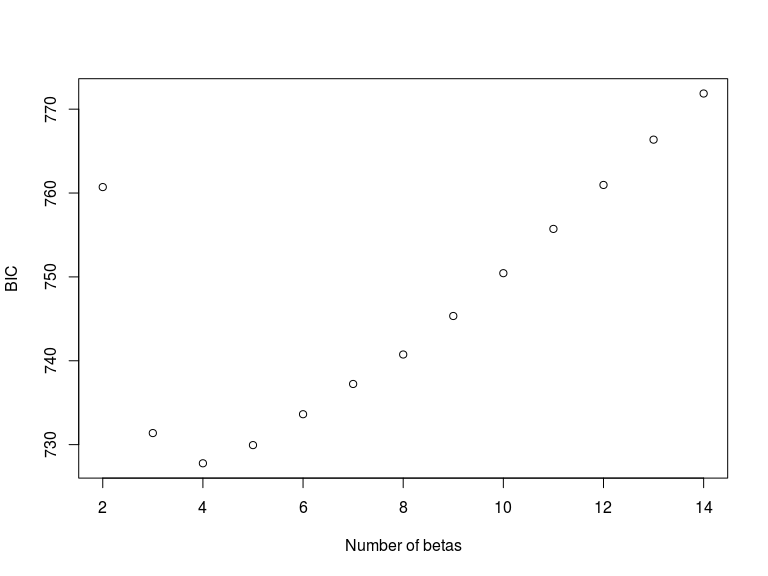
\includegraphics[width=.8\textwidth]{bic.png}}
\end{figure}

\begin{align*}
	y = & \beta_0 + \beta_1\text{AbdomenC} + \beta_2\text{Weight} + \beta_3\text{WristC} + \epsilon
\end{align*}

%====================================================================
\subsection*{Part D: Model Evaluation and Refinement}
\subsubsection*{VIF}
At this point four unique models exist that are shown below.

\begin{align*}
	y_{BWD} = & \beta_0 + \beta_1\text{AbdomenC} + \beta_2\text{Height} + \beta_3\text{NeckC} + \beta_4\text{WristC} + \epsilon \\
	y_{FWD} = & \beta_0 + \beta_1\text{AbdomenC} + \beta_2\text{Weight} + \beta_3\text{WristC} + \beta_4\text{Height} + \epsilon \\
	y_{RSS} = & \beta_0 + \beta_1\text{AbdomenC} + \beta_2\text{Height} + \beta_3\text{NeckC} + \beta_4\text{ChestC} + \beta_5\text{HipC} + \\
	&\beta_6\text{ForearmC} + \beta_7\text{WristC} + \epsilon \\
	y_{BIC} = & \beta_0 + \beta_1\text{AbdomenC} + \beta_2\text{Weight} + \beta_3\text{WristC} + \epsilon
\end{align*}

The first step taken in the model evaluation was to examine the variance inflation factors (VIF) for each unique model to determine whether or not colinearity issues are present.

The forward elimination model ($y_{FWD}$)contains two predictors with high VIF values: AbdomenC and Weight. In this model Weight has a VIF value of $\approx 9.78$; with a value near 10 it indicates issues with colinearity and was removed.

In the model chosen by Adjusted $R^2$, AbdomenC has a VIF value of $\approx 7.6$, which is significantly higher than all of the other VIF values. For this reason it was removed from the model.

The model chosen from Mallow's C and BIC contains two predictors with moderately high VIF values. For this model, AbdomenC is $\approx 4.03$ and Weight is $\approx 5.28$. Logically, it makes sense that there would be colinearity between these two predictors, but further investigation is necessary. 

After adjusting the models and re-evaluating the VIF values, the models chosen by Adjusted $R^2$ and forward elimination both have VIF values under 4 for all predictors.

\subsubsection*{Diagnostic Information}
%The R summaries for the four final models is presented below.
%
%\begin{changemargin}{-0cm}{-0cm}
%	\begin{center}
%		\lstinputlisting[language={}, caption=Backward Elimination Model Summary]{./output/lm_bwd.txt}
%	\end{center}
%\end{changemargin}
%\begin{changemargin}{-0cm}{-0cm}
%	\begin{center}
%		\lstinputlisting[language={}, caption=Forward Selection Model Summary]{./output/lm_fwd.txt}
%	\end{center}
%\end{changemargin}
%\begin{changemargin}{-0cm}{-0cm}
%	\begin{center}
%		\lstinputlisting[language={}, caption=Adjusted $R^2$ Model Summary]{./output/lm_rss.txt}
%	\end{center}
%\end{changemargin}
%\begin{changemargin}{-0cm}{-0cm}
%	\begin{center}
%		\lstinputlisting[language={}, caption=BIC Model Summary]{./output/lm_mallow.txt}
%	\end{center}
%\end{changemargin}

Examining the summaries for each model, the model chosen from the Adjusted $R^2$ method has a significantly lower adjusted $R^2$ value than any of the other models after removing the weight as a predictor ($\approx 0.54$ vs $\approx 0.71$). The other three models have very close adjusted $R^2$ values. This information is displayed below.
	\begin{center}
		\lstinputlisting[language={}, caption=Adjusted $R^2$ Values]{./output/adj_r2.txt}
	\end{center}

With the similarities between the remaining models combined with the potential colinearity issues in the BIC model, the decision was made to remove this model from consideration. If the model had a significantly higher (or even the highest) adjusted $R^2$ value out of the remaining models, further investigation would be considered. However, the forward and backward elimination models have VIF values less than 3 for all of their predictors.

Below are two sets of plots containing (from top right to bottom left): Residuals vs Fitted values, the Q-Q plot of the residuals, Residuals vs. Leverage, and the Cook's distance. The first set of plots is for the backward elimination model and the second set is for the forward selection model.

For the backward elimination model, there do not appear to be any major trends that occur in the residuals vs fitted values. Towards the higher fitted BFP values, there appears to be a reduction in variance. The Q-Q plot shows that the left and right tails are slightly light, but not extreme. Likewise, the standardized residual plot does not show any points with extreme values (absolute values larger than 3). The cooks distance plot shows that there are a few points with higher distances relative to the rest of the observations.
\begin{figure}[H]
  \begin{subfigure}[t]{.5\textwidth}
    \centering
    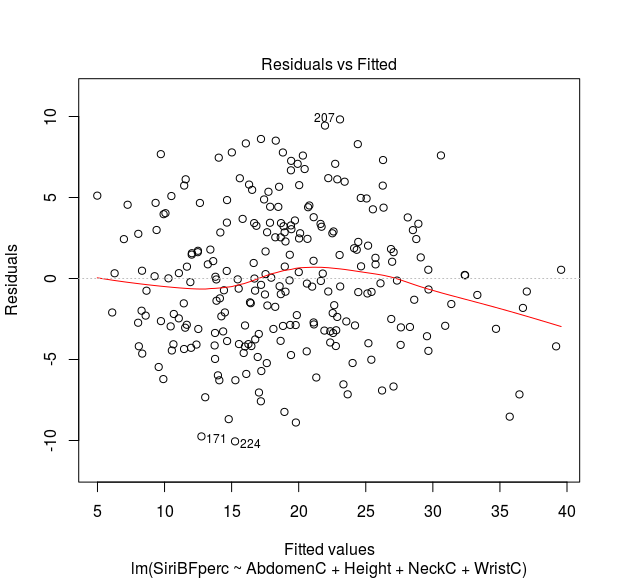
\includegraphics[width=\linewidth]{bwd_resid.png}
  \end{subfigure}
  \hfill
  \begin{subfigure}[t]{.5\textwidth}
    \centering
    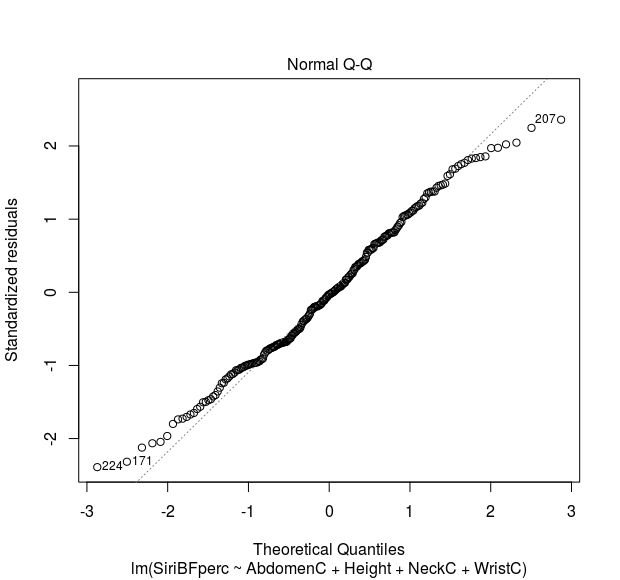
\includegraphics[width=\linewidth]{bwd_qq.png}
  \end{subfigure}
  \begin{subfigure}[t]{.5\textwidth}
    \centering
    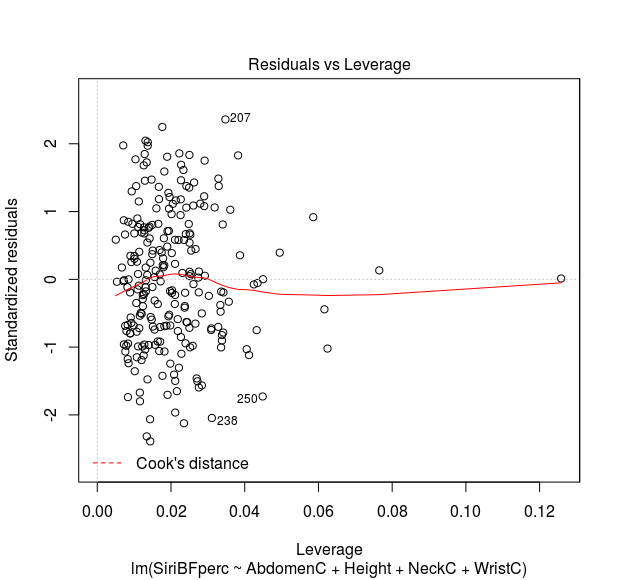
\includegraphics[width=\linewidth]{bwd_leverage.png}
  \end{subfigure}
  \hfill
  \begin{subfigure}[t]{.5\textwidth}
    \centering
    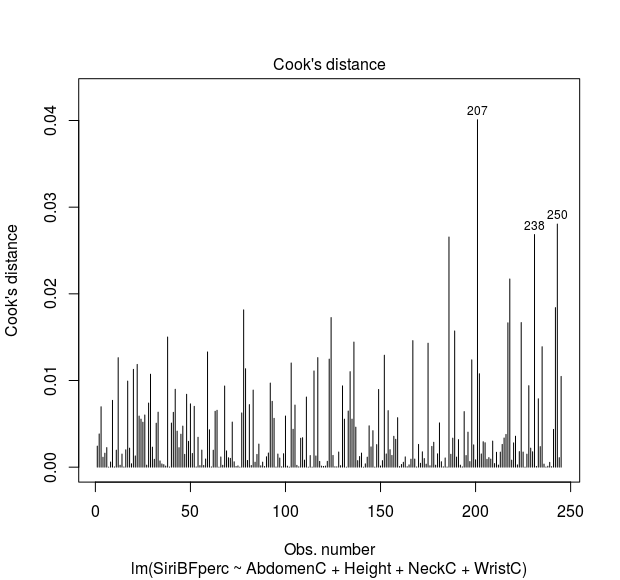
\includegraphics[width=\linewidth]{bwd_cooks.png}
  \end{subfigure}
\end{figure}

The diagnostic plots for the forward selection model show nearly identical information as the backward elimination plots.

\begin{figure}[H]
  \begin{subfigure}[t]{.5\textwidth}
    \centering
    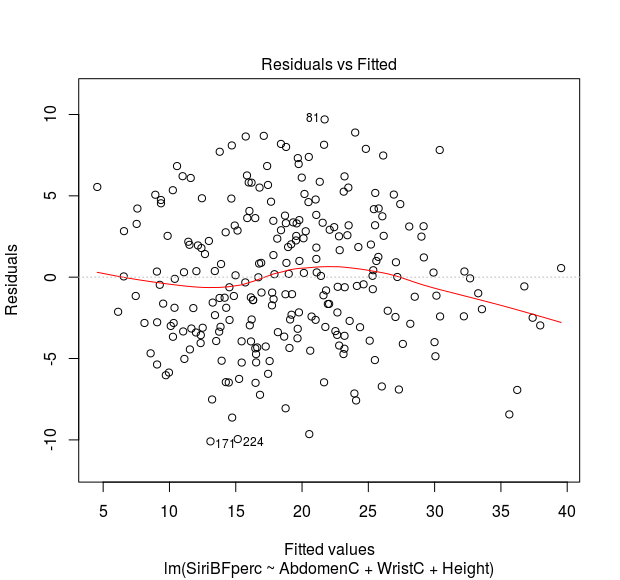
\includegraphics[width=\linewidth]{fwd_resid.png}
  \end{subfigure}
  \hfill
  \begin{subfigure}[t]{.5\textwidth}
    \centering
    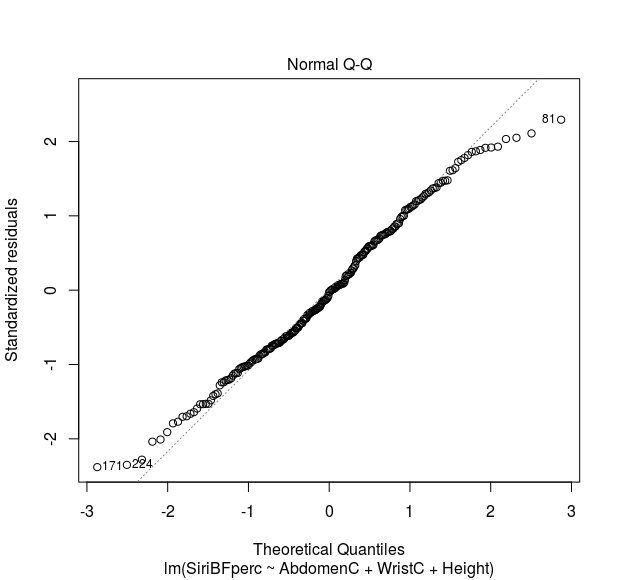
\includegraphics[width=\linewidth]{fwd_qq.png}
  \end{subfigure}
  \begin{subfigure}[t]{.5\textwidth}
    \centering
    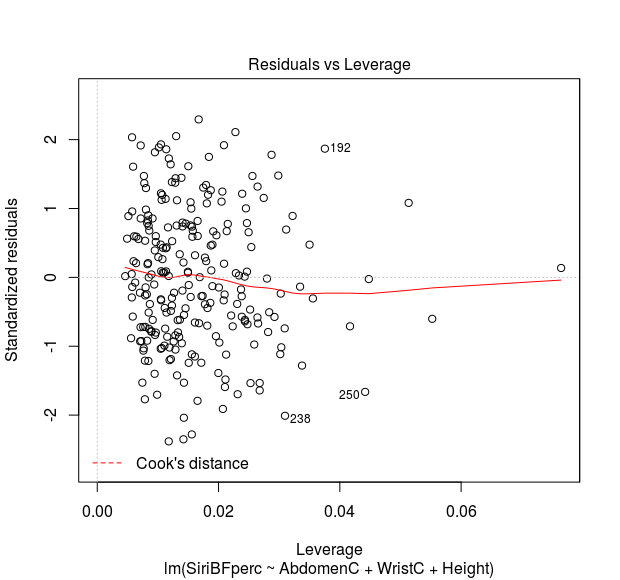
\includegraphics[width=\linewidth]{fwd_leverage.png}
  \end{subfigure}
  \hfill
  \begin{subfigure}[t]{.5\textwidth}
    \centering
    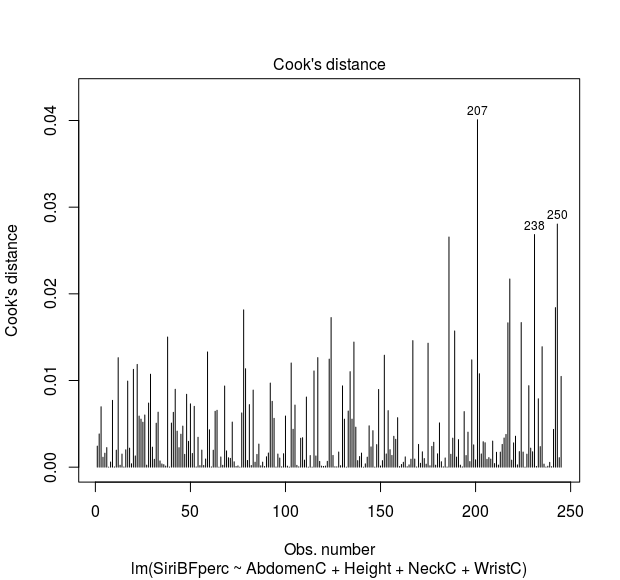
\includegraphics[width=\linewidth]{fwd_cooks.png}
  \end{subfigure}
\end{figure}

\subsubsection*{Prediction Intervals}
Due to the high similarities in the diagnostics of the two models, both models will be used to generate prediction intervals for body fat percentage. Either model may be appropriate depending on the intended usage. To compute a prediction interval about the means, the following values were obtained as the mean for every quantitative predictor used in the model:
	\lstinputlisting[language={}, caption=Mean Predictor Values]{./output/means.txt}
	
The following prediction intervals were obtained using the given mean values:
	\lstinputlisting[language={}, caption=Mean Predictor Values]{./output/predict.txt}

\subsubsection*{Final Models}
After refining the models, the following are the final model estimates
\begin{align*}
	\hat{y}_{BWD} = & 10.64971 + 0.81416\text{AbdomenC} - 0.42159\text{Height} - 0.40964\text{NeckC} - 1.17854\text{WristC}\\
	\hat{y}_{FWD} = & 8.8642 + 0.7719\text{AbdomenC} - 1.6304\text{WristC} - 0.4448\text{Height}
\end{align*}

As we can see in both models a larger abdomen circumference tends to show an increase in body fat percentage, while height and wrist circumference appear to indicate a lower body fat percentage. For the backward selection model, larger neck circumference also appears to indicate a lower body fat percentage.

%%%%%%%%%%%%%%%%%%%%%%%%%%%%%%%%%%%%%%%%%%%%%%%%%%%%%%%%%%%%%%%%%%%%
%%% SECTION: CODE APPENDIX
%%%%%%%%%%%%%%%%%%%%%%%%%%%%%%%%%%%%%%%%%%%%%%%%%%%%%%%%%%%%%%%%%%%%

%\newpage
%\section*{R Code}
%\lstinputlisting[language=R]{../hw3.r}

\end{document}
